\documentclass[11pt]{article}

\usepackage[utf8]{inputenc}
\usepackage[T1]{fontenc}
\usepackage[margin=1in]{geometry}
\usepackage{graphicx}
\usepackage{booktabs}
\usepackage{amsmath}
\usepackage{amssymb}
\usepackage[colorlinks=true,linkcolor=blue,citecolor=blue,urlcolor=blue]{hyperref}
\usepackage[round]{natbib}
\bibliographystyle{apalike}

\title{Silicon Respondents: A Latent-Conditioned Language Model that Reproduces Big Five Psychometric Structure on Unseen Items and Inventories}

% TODO: author names were not present in manuscript.md -- fill in before submission.
\author{}
\date{}

\begin{document}

\maketitle

\begin{abstract}
Large language models have been proposed as "silicon samples" --- synthetic respondents that stand in for human participants in survey and psychometric research. Existing approaches mostly prompt a model with a persona description and read back answers, which we show reproduces human factor structure only weakly. Instead, we keep an instruction-tuned model frozen and train a soft prefix and low-rank adapters that inject a continuous five-dimensional Big Five latent score obtained from real human data. We read each Likert response directly from the model's next-token digit logits, and we build a synthetic population by sampling latents from the empirical covariance of human factor scores. The resulting silicon population attains fair factor congruence with the human five-factor structure on held-out items (mean Tucker congruence $\approx$ 0.85, with four of five factors in the fair-to-good range and Neuroticism below it), and this holds when the same model is transferred to a different inventory with different items and a different response scale (IPIP$\rightarrow$BFI $\approx$ 0.86 Tucker congruence). The sign pattern of the inter-factor correlations is recovered, but their magnitude is only partially reproduced --- the Frobenius error sits above the human split-half ceiling, more so in-domain than out-of-distribution. Most importantly, the population reproduces emergent, non-injected nomological links: administered four never-seen, non-personality instruments (grit, self-esteem, leadership emergence, procrastination), it recovers the literature-documented Big Five correlates --- even though those domain$\leftrightarrow$trait relationships appear nowhere in the injected covariance. Because a generic evaluative halo can already reproduce the correlation sign pattern, we rest this claim on a discriminant multiple regression, which isolates the theoretically dominant trait with clean single-trait patterns for grit and leadership that a halo cannot produce. All results are obtained with two open-source models, Qwen2.5-1.5B-Instruct and Llama-3-8B-Instruct, running locally on a single consumer-grade GPU with a relatively small number of trainable parameters.
\end{abstract}

\section{Introduction}

A \textbf{silicon sample} uses a language model to generate synthetic respondents that stand in for a target human population \citep{argyle2023}. The appeal for behavioral research is concrete: synthetic respondents promise to lower the cost and time of data collection, to pilot instruments before fielding them on humans, to reach populations that are small, sensitive, or hard to recruit, and — most ambitiously — to serve as a testbed for \textit{scale development}, where a new questionnaire could be trialed on a synthetic pool before any human sees it \citep{grossmann2023,dillion2023}. Each of these uses treats the synthetic sample as a measurement instrument, and that framing raises a measurement question that surface plausibility does not answer: do synthetic respondents reproduce the \textit{psychometric structure} of the construct being measured, or only its marginal statistics? A model can output entirely plausible Likert numbers whose item means match a human sample, yet whose covariance does not factor into the same latent dimensions. For every use that motivates silicon sampling in the first place — factor analysis, scale authoring, criterion prediction — it is the covariance structure, not the item means, that carries the information.

This distinction is where existing evidence stops short. The silicon-sampling literature has largely validated synthetic respondents at the level of \textit{aggregate response distributions}: whether a demographically conditioned model reproduces the marginal opinion breakdown of a subpopulation \citep{argyle2023,santurkar2023}, or whether simulated agents reproduce the average outcome of a classic experiment \citep{aher2023}. In parallel, a line of work in ``LLM personality'' shows that prompting can shift a model's \textit{mean trait scores} in the intended direction and that these scores can be read off standard inventories \citep{serapiogarcia2023,jiang2023,miotto2022,pellert2024}. What neither line establishes is that a synthetic \textit{population} reproduces the inter-item covariance, factor structure, and nomological network that operationally define a psychological construct \citep{cronbachmeehl1955}. There is moreover direct reason for caution: self-report personality measurements taken from LLMs are sensitive to prompt phrasing and option ordering \citep{gupta2024}, and models exhibit a human-like social-desirability bias that inflates desirable traits once they detect they are being profiled \citep{salecha2024}. Mean-level trait recovery, in short, is both a weaker and a less trustworthy criterion than the structural one that scale developers actually depend on.

We study the structural question for the \textbf{Big Five} personality dimensions (Openness, Conscientiousness, Extraversion, Agreeableness, Neuroticism). Rather than describe a persona in the prompt, we condition a frozen instruction model on a \textit{continuous five-dimensional trait latent} through a small soft prefix and low-rank adapters, read each Likert answer directly off the model's own next-token digit logits (which preserves its language ability), and build a synthetic population by \textbf{sampling} — not taking the argmax of — those response distributions for latents drawn from the empirical human factor-score covariance. Sampling supplies the item-unique variance that psychometric structure lives in, and drawing latents from the human covariance lets the synthetic population reproduce the inter-factor correlations. We then evaluate the population not by whether its trait scores point the right way, but by whether it reproduces human factor structure on \textit{held-out items and a second inventory}, and whether it recovers documented Big Five correlates of \textit{non-personality} instruments it was never trained on.

Our contribution is this method together with a battery of validity evidence:

\begin{enumerate}
\item \textbf{Method.} A \textit{latent-conditioned} respondent simulator: a frozen instruction LM whose Likert answers are read from the model's own digit-token logits (preserving language ability), conditioned on a continuous 5-D Big Five latent through a small soft prefix and low-rank adapters, with a synthetic population built by \textbf{sampling} responses for latents drawn from the empirical human factor-score covariance.
\item \textbf{Structural validity.} The synthetic population attains fair factor congruence with the human five-factor structure on items the model never trained on (mean Tucker congruence $\approx$ 0.85, Neuroticism the weakest factor), and this transfers across inventories and response scales (IPIP$\rightarrow$BFI $\approx$ 0.86); the inter-factor correlation matrix is partially recovered --- the sign pattern is correct but its magnitude error exceeds the human split-half ceiling.
\item \textbf{Criterion/nomological validity.} The population reproduces documented Big Five correlates of \textit{non-personality} instruments (grit, self-esteem, leadership emergence, procrastination) that are absent from the injected covariance. Beyond the correlation sign pattern (which a generic evaluative halo can also reproduce), a discriminant multiple regression isolates the theoretically dominant trait — cleanly for grit and leadership — evidence that the simulator has learned construct$\rightarrow$response behaviour rather than replaying an injected correlation matrix or an evaluative halo.
\item \textbf{Robustness.} Replication across five seeds and a second, larger backbone (Llama-3-8B), together with held-out temperature calibration and silicon generative (sampling) stability, establishes that the headline numbers are not single-run or hyperparameter artifacts.
\end{enumerate}

We position this against prompt-persona approaches \citep{serapiogarcia2023,jiang2023}, which we include as zero-shot baselines and over which trained latent conditioning roughly doubles factor congruence, and against the broader debate on whether LLMs can substitute for human participants \citep{dillion2023,bisbee2024}. We are also explicit about the limit of the design: the conditioning latents are CFA factor scores derived from the training inventory and the inter-factor covariance is injected by construction, so a degree of circularity is built in — which is precisely why the emergent, non-injected criterion validity of \S{}5.4 --- in particular its discriminant regression analysis, which a generic evaluative halo cannot satisfy --- carries the weight of the argument.


\section{Related work}

\subsection{Silicon samples: language models as synthetic respondents}

The proposal to use language models as stand-ins for human respondents originates with \citet{argyle2023}, who condition GPT-3 on demographic backstories and show it reproduces aggregate response patterns of the corresponding subpopulations — a property they term \textit{algorithmic fidelity}. The idea has since been pursued across disciplines: as \textit{homo silicus} in economics, where models given endowments and preferences reproduce classic behavioral-economics findings \citep{horton2023}; as ``Turing experiments'' that replicate the average outcomes of canonical psychology and psycholinguistics studies \citep{aher2023}; as memory-augmented generative agents that enact believable day-to-day behavior \citep{park2023}; and as a general prospect for social-science research \citep{grossmann2023}. A parallel strand probes whose opinions a model actually reflects, finding systematic misalignment between model outputs and the demographic groups they are meant to represent \citep{santurkar2023}. Critical work cautions that synthetic samples can distort distributions and correlations relative to humans and warns against treating them as drop-in replacements \citep{bisbee2024,dillion2023}. What unites these efforts — supportive and critical alike — is that they evaluate fidelity at the level of \textit{aggregate or marginal} response patterns: the marginal breakdown of an opinion item, or the mean outcome of an experiment. The quantity a scale developer cares about — whether the synthetic responses factor into the same latent structure as human data — is left untested. We take that structural reproduction, on held-out items and across inventories, as the object of study.

\subsection{Simulating personality and personas in language models}

A second line of work asks whether LLMs can be made to express a target \textit{personality}. Prompting a model with a persona or a trait description reliably shifts its self-reported Big Five scores in the intended direction, and these scores can be elicited with standard human inventories \citep{serapiogarcia2023,jiang2023,miotto2022}; broader psychometric batteries extend the same idea to values, clinical, and interpersonal scales \citep{pellert2024,huang2024}. These studies establish that trait \textit{scores} are steerable and measurable, but two findings caution against reading them as evidence of construct-valid personality. First, LLM self-reports are unstable: semantically equivalent prompts and reordered response options produce significantly different trait scores, so the measurement itself is unreliable \citep{gupta2024}. Second, models display a human-like social-desirability bias, skewing toward desirable trait poles once they infer that a personality assessment is underway \citep{salecha2024} — the same evaluative halo we must guard against in our own criterion analysis (\S{}5.4). Our approach departs from this line in two ways: we replace the free-text persona with a \textit{trained, continuous latent} that is fit to human factor scores rather than described in words, and we validate at the level of population factor structure and nomological network rather than mean trait recovery, sidestepping the prompt-sensitivity failure mode by never phrasing the trait as a natural-language instruction.

\subsection{Construct validity as the evaluation bar}

We hold the generation of synthetic population to the psychometric notion of \textit{construct validity}: a construct is defined not by any single indicator but by its place in a \textit{nomological network} of relationships to other measures \citep{cronbachmeehl1955}. Reproducing a construct therefore means reproducing (i) its internal structure — the factor pattern and inter-item covariance, for which we use Tucker's congruence coefficient \citep{tucker1951,lorenzoseva2006} and Cronbach's $\alpha$ \citep{cronbach1951} — and (ii) its external relationships, for which we use meta-analytically documented Big Five correlates of grit \citep{duckworth2009}, self-esteem \citep{rosenberg1965,robins2001}, leadership emergence \citep{judge2002}, and procrastination \citep{steel2007} as criterion targets. This is a strictly more demanding bar than the mean-trait-recovery criterion of the personality-prompting literature: a model can shift its trait scores correctly while failing to reproduce either the factor structure or the nomological links, and it is precisely those latter properties that determine whether a synthetic sample is usable for factor-analytic scale development.

\subsection{Conditioning mechanisms}

Injecting a dense trait code into a frozen backbone is a parameter-efficient fine-tuning problem. We combine soft prefixes / prompt tuning \citep{lester2021} with low-rank adapters (LoRA) \citep{hu2021} and read answers generatively off the digit logits, keeping the language head intact so the same model can also produce free text. This is a distinct design point from inference-time activation steering, in which a trait or behavior direction is added to hidden states without training a mapping from a continuous construct latent to responses \citep{zou2023}. Steering shows that trait-like directions exist in a model's representation space; our aim is different — to \textit{learn} a construct$\rightarrow$response mapping whose synthetic outputs reproduce human psychometric structure — and the soft-prefix-plus-LoRA path lets us fit that mapping from human factor scores while leaving the readout generative.


\section{Method}
\label{sec:method}

\subsection{Overview and notation}
\label{sec:overview}

We model a questionnaire respondent as a conditional distribution over Likert responses. Let $\mathbf{z} = (z_O, z_C, z_E, z_A, z_N)^\top \in \mathbb{R}^5$ denote a respondent's standing on the five personality factors, expressed as standardized factor scores; let $x_j$ denote the text of item $j$; and let $Y_{ij} \in \{1, \dots, K\}$ denote the Likert response of respondent $i$ to item $j$ (the training inventory uses $K = 5$). The simulator defines a conditional categorical response distribution
\begin{equation}
p_\theta\!\left(Y_{ij} = k \mid x_j, \mathbf{z}_i\right), \qquad k = 1, \dots, K,
\label{eq:model}
\end{equation}
parameterized by a frozen, instruction-tuned language model augmented with a small set of trainable conditioning modules, collectively denoted $\theta$. A synthetic respondent population --- a \textit{silicon sample} --- is then obtained in two steps: latent vectors $\mathbf{z}_i$ are drawn from the empirical distribution of human factor scores, and each synthetic respondent's item responses are sampled from Equation~\ref{eq:model} (Section~\ref{sec:silicon}). Figure~\ref{fig:architecture} gives an overview of the architecture; the following subsections define each component.

\begin{figure}[t!]
\centering
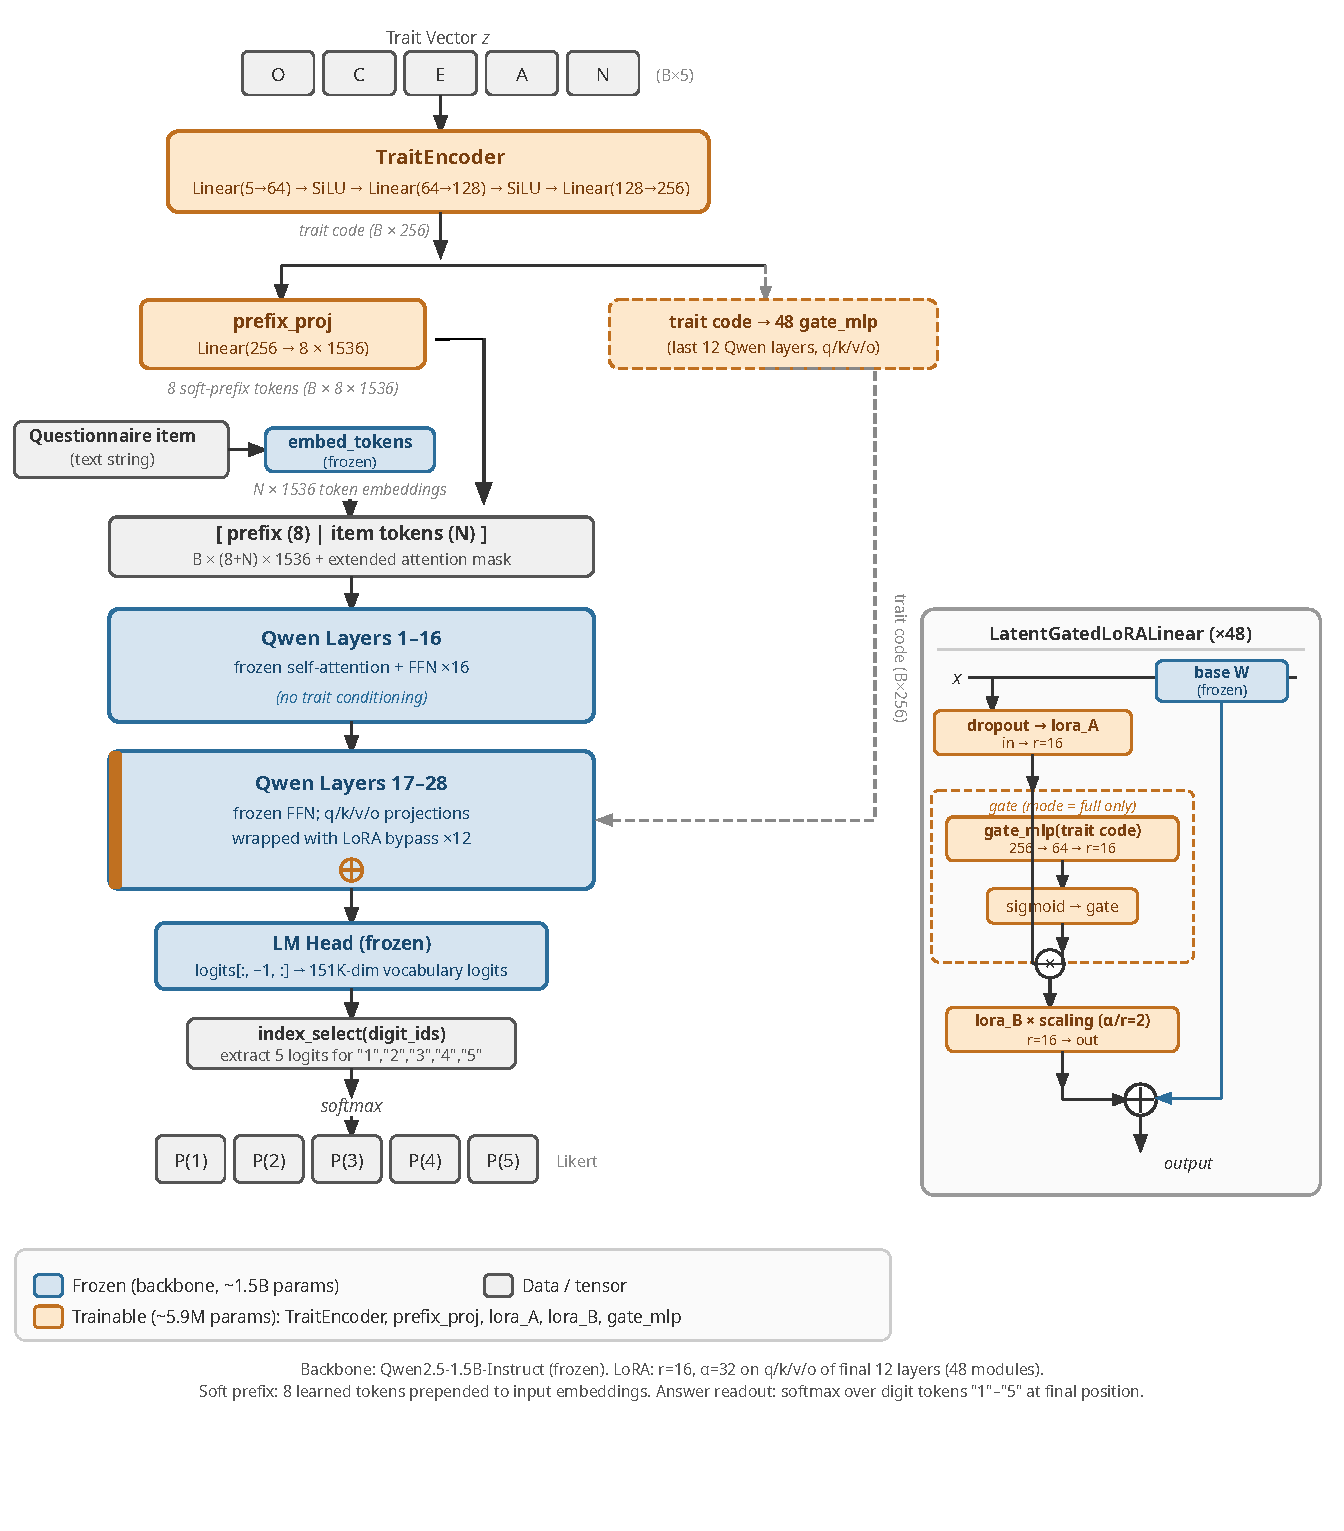
\includegraphics[width=0.92\linewidth]{figures/architecture.pdf}
\caption{Architecture of the respondent simulator (shown for the Qwen2.5-1.5B backbone). Blue components belong to the frozen backbone ($\approx$1.5B parameters, including the token embeddings and the language-modeling head); orange components are the trainable conditioning modules ($\approx$5.9M parameters): the trait encoder $E_\phi$ (Equation~\ref{eq:traitcode}), the prefix projection, and the latent-gated low-rank adapters wrapped around the query/key/value/output projections of the final 12 transformer layers. The five-dimensional latent $\mathbf{z}$ is encoded into a 256-dimensional trait code that (i) produces $m = 8$ soft prefix embeddings prepended to the item's token embeddings and (ii) drives the per-rank sigmoid gates of the 48 adapter modules (inset: a single wrapped projection, Equation~\ref{eq:lora}). The Likert response distribution is read from the final-position next-token logits restricted to the digit tokens ``1''--``5'' (Equation~\ref{eq:readout}). The dashed gate path is active only in the \textit{full} condition; the ungated ablation fixes $\mathbf{g} = \mathbf{1}$ (Section~\ref{sec:baselines}).}
\label{fig:architecture}
\end{figure}

\subsection{Backbone and generative Likert readout}
\label{sec:readout}

The backbone is a frozen, instruction-tuned, causal language model. We used two relatively small Llms, that can run on a commercial GPU, in our case a Nvidia RTX 4090 with 24gb of memory:  Qwen2.5-1.5B-Instruct; Llama-3-8B-Instruct (4-bit quantized) . All backbone parameters --- token embeddings, transformer layers, and the language-modeling head --- remain frozen throughout training and evaluation.

Each item is presented in the backbone's chat format with the system message ``You are a psychometric respondent simulator.'' and a user turn containing the item text followed by the instruction ``On a scale of 1 to 5 (1 = Strongly Disagree, 5 = Strongly Agree), how much do you agree? Answer with a single number.'' Let $\boldsymbol{\ell} \in \mathbb{R}^{|\mathcal{V}|}$ denote the next-token logits produced by the frozen language-modeling head at the final position of this prompt, where $\mathcal{V}$ is the vocabulary, and let $t_1, \dots, t_5$ index the vocabulary entries of the digit tokens ``1'' through ``5''. The response distribution is the temperature-scaled softmax restricted to these five tokens:
\begin{equation}
p_\theta\!\left(Y = k \mid x, \mathbf{z}\right) \;=\; \frac{\exp\!\left(\ell_{t_k} / T\right)}{\sum_{k'=1}^{5} \exp\!\left(\ell_{t_{k'}} / T\right)},
\label{eq:readout}
\end{equation}
where $T > 0$ is a sampling temperature ($T = 1$ during training; its role at generation time is examined in \S{}5.5). This generative readout was chosen over a dedicated classification head for two reasons. First, because the answer is produced by the model's own language-modeling head, the model retains its full generative ability and can also produce open-ended text under the same trait conditioning (\S{}5.7). Second, Equation~\ref{eq:readout} yields a proper categorical distribution for every (item, respondent) pair, which can be \textit{sampled}; Section~\ref{sec:silicon} explains why sampling, rather than taking the modal response, is essential for reproducing psychometric structure.

\subsection{Latent conditioning}
\label{sec:conditioning}

The latent $\mathbf{z}$ is injected into the frozen backbone through two trainable, parameter-efficient paths that share a common representation. A trait encoder $E_\phi$ --- a three-layer perceptron ($5 \to 64 \to 128 \to 256$, SiLU activations) --- first maps the latent to a trait code
\begin{equation}
\mathbf{c} \;=\; E_\phi(\mathbf{z}) \;\in\; \mathbb{R}^{256}.
\label{eq:traitcode}
\end{equation}

\paragraph{Path 1: soft prefix.} An affine projection maps the trait code to $m = 8$ continuous prefix embeddings,
\begin{equation}
\mathbf{P} \;=\; \operatorname{reshape}\!\left(\mathbf{W}_{\!P}\,\mathbf{c} + \mathbf{b}_P\right) \;\in\; \mathbb{R}^{m \times d},
\label{eq:prefix}
\end{equation}
which are prepended to the item's token-embedding sequence, $[\,\mathbf{P};\, \mathbf{E}_{\text{emb}}(x_j)\,]$, with the attention mask extended accordingly \citep{lester2021}. The projection weights are initialized with small variance ($\mathcal{N}(0, 0.02^2)$, zero bias), so at the start of training the prefix is close to a null input and the conditioned model's behavior starts near that of the unconditioned backbone.

\paragraph{Path 2: latent-gated low-rank adaptation.} Each of the query, key, value, and output projections in the self-attention blocks of the final 12 (of 28) transformer layers --- 48 modules in total --- is wrapped with a low-rank adapter \citep{hu2021} of rank $r = 16$ and scaling $\alpha = 32$. Writing $\mathbf{W}_0$ for the frozen projection weight and $\mathbf{u}$ for its input, the wrapped projection computes
\begin{equation}
\mathbf{h} \;=\; \mathbf{W}_0 \mathbf{u} \;+\; \frac{\alpha}{r}\, \mathbf{B}\left(\mathbf{g} \odot \mathbf{A}\tilde{\mathbf{u}}\right), \qquad \mathbf{g} \;=\; \sigma\!\left(G_\psi(\mathbf{c})\right) \in (0,1)^r,
\label{eq:lora}
\end{equation}
where $\mathbf{A} \in \mathbb{R}^{r \times d_{\text{in}}}$ and $\mathbf{B} \in \mathbb{R}^{d_{\text{out}} \times r}$ are trainable ($\mathbf{B}$ is zero-initialized, so the bypass initially contributes nothing), $\tilde{\mathbf{u}}$ is the input after dropout ($p = .05$), $G_\psi$ is a two-layer gate network ($256 \to 64 \to r$, SiLU), $\sigma$ is the logistic function, and $\odot$ denotes elementwise multiplication. The gate $\mathbf{g}$ modulates each of the $r$ bottleneck dimensions as a function of the trait code, allowing the adapter's effective update to vary with the respondent's trait profile. Fixing $\mathbf{g} = \mathbf{1}$ recovers standard (ungated) LoRA; this ungated variant is evaluated as an ablation, and --- anticipating \S{}5.3 --- the gate confers no reliable advantage, so we do not claim it as a contribution of the method.

Across the trait encoder, prefix projection, adapters, and gate networks, approximately 5.9M parameters are trainable for the Qwen backbone --- roughly 0.4\% of the backbone's parameter count. Everything else is frozen.

\subsection{Training data and objective}
\label{sec:training}

Training data are item-level responses from the IPIP-50 Big Five inventory ($N = 15{,}775$ participants). Each participant's latent $\mathbf{z}_i$ is their vector of factor scores from a confirmatory five-factor model fitted to the human data (Section~\ref{sec:instruments} describes the item partitions; 30 of the 50 items are used for training and 20 --- four per factor --- are withheld entirely). With $\mathcal{D}$ the set of observed (participant, item) response pairs over the training items, the trainable modules minimize the negative log-likelihood of the observed responses under Equation~\ref{eq:readout} at $T = 1$:
\begin{equation}
\mathcal{L}(\theta) \;=\; -\,\frac{1}{|\mathcal{D}|} \sum_{(i,j) \in \mathcal{D}} \log p_\theta\!\left(Y = y_{ij} \mid x_j,\, \mathbf{z}_i + \boldsymbol{\varepsilon}_{ij}\right), \qquad \boldsymbol{\varepsilon}_{ij} \sim \mathcal{N}\!\left(\mathbf{0},\, \sigma_\varepsilon^2 \mathbf{I}_5\right),
\label{eq:loss}
\end{equation}
where the isotropic jitter $\boldsymbol{\varepsilon}_{ij}$ ($\sigma_\varepsilon = 0.1$, redrawn at every presentation) regularizes the conditioning channel against overfitting to exact factor-score values; validation uses unperturbed latents. Optimization uses AdamW (learning rate $2 \times 10^{-4}$, weight decay 0.01), batch size 16, three epochs, and a schedule of 3\% linear warmup followed by cosine decay, in bfloat16 precision. Model selection is by cross-entropy on responses to the 20 held-out items, so the selected checkpoint is the one that best generalizes beyond the items seen in the loss rather than the one that best fits the training items. Because selection is by pointwise per-item cross-entropy whereas the reported structural metric is factor congruence (a second-order property of the item correlation matrix), the resulting selection bias on the \S{}5.1 held-out estimate is minimal; moreover, the cross-inventory (\S{}5.2) and criterion (\S{}5.4) results, which do not inform checkpoint selection at all, corroborate that estimate.


\subsection{Constructing a silicon sample}
\label{sec:silicon}

A silicon sample of $n$ synthetic respondents is generated in two steps.

\begin{enumerate}
\item \textbf{Population latents.} Respondent latents are drawn from a multivariate normal matched to the human factor-score distribution,
\begin{equation}
\mathbf{z}_i \;\overset{\text{iid}}{\sim}\; \mathcal{N}_5\!\left(\boldsymbol{\mu}_{\text{human}},\, \Sigma_{\text{human}}\right), \qquad i = 1, \dots, n,
\label{eq:latents}
\end{equation}
where $\boldsymbol{\mu}_{\text{human}}$ and $\Sigma_{\text{human}}$ are the empirical mean vector and covariance matrix of the human CFA factor scores. Because $\Sigma_{\text{human}}$ encodes the human inter-factor covariance, the synthetic population reproduces the inter-factor correlation structure $\Phi$ \textit{at the latent level} by construction; whether that structure survives the mapping into item responses is an empirical question (\S{}5.1).
\item \textbf{Response sampling.} Each synthetic respondent answers every administered item by sampling from the model's categorical at temperature $T$,
\begin{equation}
Y_{ij} \;\sim\; \operatorname{Categorical}\!\left(p_\theta(\,\cdot \mid x_j, \mathbf{z}_i)\right).
\label{eq:sampling}
\end{equation}
\end{enumerate}

Sampling, rather than taking the modal response $\arg\max_k p_\theta(k \mid x_j, \mathbf{z}_i)$, is essential: the argmax collapses each respondent--item distribution to a deterministic function of $\mathbf{z}$, discarding the item-unique variance on which factor analysis operates (in the pilot design, argmax readout reduced mean per-item response variance to 0.96, against 1.42 in the human data). Unless stated otherwise, the administered items are the \textit{held-out} items, so all structural results concern items the model never saw during training.

\subsection{Baseline and ablation conditions}
\label{sec:baselines}

Four conditioning modes form a ladder from no trait information to the full trained method:

\begin{enumerate}
\item \textit{baseline\_a} (floor): the frozen backbone answers each item with no trait information of any kind.
\item \textit{baseline\_b} (persona prompt): the frozen backbone receives the trait profile as text in the prompt --- either the numeric $z$-scores or a verbal rendering into ordinal labels --- and is instructed to answer as that person would. No weights are trained. This operationalizes the prompt-persona approach of prior work \citep{argyle2023,serapiogarcia2023,jiang2023}; the exact prompt formats are given in \S{}5.3.
\item \textit{baseline\_c} (trained, ungated): the soft prefix and adapters of Section~\ref{sec:conditioning} are trained with the gate disabled ($\mathbf{g} = \mathbf{1}$ in Equation~\ref{eq:lora}).
\item \textit{full} (trained, gated): identical to \textit{baseline\_c} plus the trained gate networks $G_\psi$.
\end{enumerate}

The two trained conditions share the training protocol of Section~\ref{sec:training}. Each trained checkpoint is always evaluated under the conditioning mode it was trained with.


\section{Evaluation methodology}
\label{sec:evaluation}

\subsection{Instruments and data partitions}
\label{sec:instruments}

Three evaluation sets probe increasingly distant generalization from the training data.


\paragraph{IPIP held-out items.} The 50 IPIP items were partitioned at the item level, stratified by factor: 30 items for training and 20 never-trained items (four per factor) constituting the new-item test. Throughout, we use held-out and new-item to mean never present in the training objective, i.e. the model's weights are never updated on these items; note that the 20 held-out items are additionally used for checkpoint selection (Section~\ref{sec:training}), so they are held out from the training loss but not from model selection. A separate participant-holdout set (the 30 training items answered by 3,944 additional participants not used in training) supports a well-powered structural check on seen items.


\paragraph{BFI (out-of-distribution inventory).} A second inventory, the Big Five Inventory (25 items, five per factor; 2,800 human respondents), tests cross-inventory transfer: the items share no wording with the IPIP, and the human data were collected on a 1--6 response scale rather than 1--5. Item stems were reworded to first person to match the phrasing convention of the training items. Silicon respondents answer all instruments through the five-point readout of Equation~\ref{eq:readout}; because every comparison metric below is correlation- or covariance-based, the scale difference between silicon (1--5) and human BFI (1--6) responses is immaterial.

\paragraph{Criterion battery.} A four-instrument battery from outside the personality domain (grit, self-esteem, leadership emergence, procrastination), used for the nomological-validity analyses, is described together with its analysis in \S{}5.4.

\subsection{Psychometric indices}
\label{sec:indices}

Human and silicon response matrices are analyzed identically in R (packages \textit{psych} and \textit{GPArotation}): a five-factor exploratory factor analysis (minimum-residual extraction, oblimin rotation) is fitted separately to each matrix, and the resulting solutions are compared on four indices.

\paragraph{Factor congruence.} Let $\boldsymbol{\lambda}^{H}$ and $\boldsymbol{\lambda}^{S}$ denote the loading vectors of a matched human and silicon factor over the $p$ common items. Factor similarity is quantified by Tucker's congruence coefficient \citep{tucker1951},
\begin{equation}
\varphi\!\left(\boldsymbol{\lambda}^{H}, \boldsymbol{\lambda}^{S}\right) \;=\; \frac{\sum_{j=1}^{p} \lambda^{H}_{j}\, \lambda^{S}_{j}}{\sqrt{\left(\sum_{j=1}^{p} \bigl(\lambda^{H}_{j}\bigr)^{2}\right)\left(\sum_{j=1}^{p} \bigl(\lambda^{S}_{j}\bigr)^{2}\right)}},
\label{eq:tucker}
\end{equation}
with factors matched one-to-one by a greedy assignment on the congruence matrix. The mean of Equation~\ref{eq:tucker} over the five matched factors is the headline structural index; values of .85--.94 are conventionally read as fair similarity and $\geq$ .95 as factor equality \citep{lorenzoseva2006}.

\paragraph{Inter-factor structure.} The oblimin factor-correlation matrices $\Phi^{H}$ and $\Phi^{S}$ are compared by the Frobenius norm of their difference, $\lVert \Phi^{S} - \Phi^{H} \rVert_F$ (lower is better).

\paragraph{Internal consistency and item behavior.} For each trait scale of $k$ items with item variances $\sigma^2_j$ and total-score variance $\sigma^2_X$, Cronbach's alpha \citep{cronbach1951},
\begin{equation}
\alpha \;=\; \frac{k}{k-1}\left(1 - \frac{\sum_{j=1}^{k} \sigma^2_j}{\sigma^2_X}\right),
\label{eq:alpha}
\end{equation}
is computed for human and silicon data and compared as $\lvert \alpha^{S} - \alpha^{H} \rvert$, alongside corrected item--total correlations (each item against the sum of the remaining items of its scale) and the eigenvalue spectra of the item correlation matrices.

The full pipeline was validated by splitting the human sample into two disjoint random halves and comparing them with the identical factor-analysis machinery, run separately on each evaluation item set (the 20 held-out IPIP items, four per factor; and the 25 BFI items, five per factor). Because the halves are independent subsamples of one population analysed on exactly the items used for the silicon comparison, this establishes an item-set--matched human noise ceiling for each metric: mean Tucker congruence 0.988 (IPIP; every factor including Neuroticism at 0.98--0.99, $n \approx 1{,}972$ per half) and 0.974 (BFI), with a $\Phi$ Frobenius error of 0.200 and 0.192 respectively and per-scale alphas agreeing to within 0.04. The IPIP ceiling is particularly informative: because it is computed on the same four-items-per-factor partition used for the held-out silicon test, it shows that four items per factor is no obstacle to near-perfect congruence between two human samples, so any silicon shortfall on that partition cannot be attributed to factor-analytic sampling noise from the small item count. These are the strongest values any silicon population could realistically attain given ordinary sampling variability, so a silicon result approaching this ceiling indicates the simulator rather than the analysis pipeline is the limiting factor; conversely, a residual $\Phi$ error of $\approx 0.2$ is expected even between two groups of humans and should be read as the baseline against which silicon $\Phi$ errors are judged.



\section{Results}

\subsection{Factor-structure reproduction (held-out items)}

Table 1 reports IPIP held-out performance (20 items, 4 per factor) aggregated by backbone. Qwen-2.5-1.5B achieves a mean Tucker congruence of 0.850 $\pm$ 0.014. Replication is tightest for Conscientiousness (0.90 $\pm$ 0.02) and Agreeableness (0.88 $\pm$ 0.01) and loosest for Neuroticism (0.74 $\pm$ 0.05) and Extraversion (0.84 $\pm$ 0.03). Llama-3-8B-4bit reaches 0.873 $\pm$ 0.034, with particularly high Extraversion (0.94 $\pm$ 0.02) and Conscientiousness (0.91 $\pm$ 0.03); Openness and Neuroticism show wider cross-seed variance (SDs 0.06 and 0.08 respectively). The $\Phi$ Frobenius error and mean corrected item-total correlation are comparable across backbones, and the silicon item-total correlation (0.481 Qwen, 0.494 Llama) closely matches the human value of 0.484 (Table 1).

\begin{table}[ht!]
\centering
\caption{Tucker congruence coefficients and related psychometric indices for the IPIP held-out set (20 items, 4 per factor). Tucker: mean Tucker congruence across the five matched factors. O–N: per-factor Tucker congruence for Openness (O), Conscientiousness (C), Extraversion (E), Agreeableness (A), and Neuroticism (N). $\Phi$ error: Frobenius norm of the difference between the silicon and human inter-factor correlation matrices. item-r: mean corrected item-total correlation over the held-out items (human reference 0.484). All values are mean $\pm$ SD across five seeds. SD reflects cross-seed variability in how consistently each factor is recovered.}
\resizebox{\textwidth}{!}{%
\begin{tabular}{lcccccccc}
\toprule
Group & Tucker & O & C & E & A & N & $\Phi$ error & item-r \\
\midrule
Qwen  & 0.850 $\pm$ 0.014 & 0.90 $\pm$ 0.01 & 0.90 $\pm$ 0.02 & 0.84 $\pm$ 0.03 & 0.88 $\pm$ 0.01 & 0.74 $\pm$ 0.05 & 0.640 $\pm$ 0.060 & 0.481 $\pm$ 0.024 \\
Llama  & 0.873 $\pm$ 0.034 & 0.89 $\pm$ 0.06 & 0.91 $\pm$ 0.03 & 0.94 $\pm$ 0.02 & 0.87 $\pm$ 0.03 & 0.76 $\pm$ 0.08 & 0.729 $\pm$ 0.103 & 0.494 $\pm$ 0.028 \\
\bottomrule
\end{tabular}
}
\end{table}

\textbf{Inter-factor structure.} The sign pattern of the human inter-factor correlations is recovered (E–A positive, C–N negative, E–N negative), but its magnitude is only partially reproduced. The $\Phi$ Frobenius error is 0.640 $\pm$ 0.060 (Qwen) and 0.729 $\pm$ 0.103 (Llama) — roughly three times the item-set-matched human split-half ceiling of 0.200 on these same 20 items (\S\ref{sec:indices}). Inter-factor structure is thus the weakest aspect of the held-out result; it is reproduced more closely out of distribution on the BFI (\S{}5.2). We therefore do not claim that the inter-factor matrix is preserved, only that its qualitative sign structure is.

\textbf{The shortfall is genuine, not sampling noise, and concentrated in Neuroticism.} Because a five-factor EFA on only four items per factor might in principle be unstable, we read the held-out numbers against the human split-half ceiling computed on the identical 20 items, four per factor (\S\ref{sec:indices}): two disjoint human subsamples ($n \approx 1{,}972$ each) reproduce each other at mean Tucker 0.988, with every factor — Neuroticism included — at 0.98–0.99 and $\Phi$ error 0.200. Four items per factor is therefore not an obstacle to near-perfect congruence between two human samples, so the silicon shortfall (mean 0.85; Neuroticism 0.74–0.76) reflects the simulator rather than factor-analytic sampling noise, and it is concentrated in Neuroticism. A separate well-powered check on \emph{seen} items — 30 items, six per factor, new synthetic respondents — reaches mean Tucker 0.986 with all five factors at 0.98–0.99 and $\Phi$ error 0.224; but because these items enter the training loss, this demonstrates only that the conditioning \emph{can} represent the full five-factor structure for in-distribution items, and does not bear on the held-out gap, which the matched ceiling above shows to be real.

\subsection{Cross-inventory transfer (BFI, out of distribution)}

Table 2 reports performance on the 25 BFI items (different inventory, different wording, 1–6 scale) — items the model never saw during training. Qwen achieves a mean Tucker congruence of 0.871 $\pm$ 0.017, with uniformly high Openness (0.93 $\pm$ 0.02) and Agreeableness (0.89 $\pm$ 0.02); Neuroticism is the weakest factor (0.76 $\pm$ 0.06). Llama reaches 0.843 $\pm$ 0.061.

Taken together, both backbones transfer to a completely different instrument with different item wording and a different response scale (1–6 vs 1–5), which can only arise if the model has learned construct-to-response behaviour rather than surface item features. The $\Phi$ Frobenius error ($\approx$0.40 for both backbones) is in fact smaller than on the IPIP held-out items ($\approx$0.64--0.73), though still about twice the BFI human split-half ceiling of 0.192 (\S\ref{sec:indices}); inter-factor structure is thus recovered somewhat better out of distribution than in domain, but on neither set does it reach the human ceiling. The mean corrected item-total correlation ($\approx$0.42) is close to, though slightly below, both the IPIP value ($\approx$0.48) and the human BFI reference of 0.500 (Table 2 vs Table 1). Anyway, we analyze in section \S{}5.6 the role of Temperature and found that Tucker congruence is nonetheless robust to temperature choice.

\begin{table}[ht!]
\centering
\caption{Tucker congruence coefficients and related psychometric indices for the BFI out-of-distribution set (25 items, 5 per factor). Column definitions as in Table 1 (item-r human reference 0.500).}
\resizebox{\textwidth}{!}{%
\begin{tabular}{lcccccccc}
\toprule
Group & Tucker & O & C & E & A & N & $\Phi$ error & item-r \\
\midrule
Qwen  & 0.871 $\pm$ 0.017 & 0.93 $\pm$ 0.02 & 0.88 $\pm$ 0.01 & 0.90 $\pm$ 0.01 & 0.89 $\pm$ 0.02 & 0.76 $\pm$ 0.06 & 0.403 $\pm$ 0.059 & 0.420 $\pm$ 0.011 \\
Llama  & 0.843 $\pm$ 0.061 & 0.93 $\pm$ 0.01 & 0.76 $\pm$ 0.09 & 0.84 $\pm$ 0.11 & 0.88 $\pm$ 0.04 & 0.81 $\pm$ 0.07 & 0.409 $\pm$ 0.063 & 0.418 $\pm$ 0.026 \\
\bottomrule
\end{tabular}
}
\end{table}

\subsection{Baselines and ablation ladder}

We evaluate four conditioning modes that form a ladder from no trait information to the full trained method. All modes share the same system prompt ("You are a psychometric respondent simulator.") and the same Likert instruction appended to the user turn ("On a scale of 1 to 5 (1 = Strongly Disagree, 5 = Strongly Agree), how much do you agree? Answer with a single number."). They differ in whether and how the Big Five latent z = (O, C, E, A, N) is communicated to the model.

Baseline\_a (floor) uses the frozen backbone with no trait information — the item text is the sole content of the user turn. No weights are updated. This measures what psychometric structure a general instruction model produces when answering personality items without any conditioning.

Baseline\_b (persona prompt) keeps the backbone frozen and injects the trait profile as text in the user turn. Two formats are tested. In the numeric style the latent z-scores are prepended as a header block:

\begin{verbatim}
Participant Profile
Openness: 0.72
Conscientiousness: -0.34
Extraversion: 1.05
Agreeableness: 0.18
Neuroticism: -0.82

Question: [item text]
On a scale of 1 to 5 ...
\end{verbatim}

In the verbal style the z-scores are first mapped to ordinal labels (z $\geq$ 1.0 $\rightarrow$ "very high"; 0.5 $\leq$ z < 1.0 $\rightarrow$ "high"; $-$0.5 < z < 0.5 $\rightarrow$ "average"; $-$1.0 < z $\leq$ $-$0.5 $\rightarrow$ "low"; z $\leq$ $-$1.0 $\rightarrow$ "very low") and the prompt opens with a role-play instruction:

\begin{verbatim}
You are role-playing a specific person with this personality profile (Big Five):
- Openness: high
- Conscientiousness: average
- Extraversion: very high
- Agreeableness: average
- Neuroticism: low

Answer the question as this person would.

Question: [item text]
On a scale of 1 to 5 ...
\end{verbatim}

No weights are updated in either variant; the model relies entirely on its instruction-following prior to interpret the profile.

Baseline\_c (trained, no gate) fine-tunes the soft prefix and LoRA adapters described in Section~\ref{sec:conditioning}, with the gate MLP disabled. The text prompt reverts to the baseline\_a format — no numeric or verbal profile appears in the prompt — because the trait information is delivered entirely through the 8 continuous prefix tokens prepended to the input embeddings. Three training epochs, item-holdout model selection.

Full (trained, gated LoRA) is identical to baseline\_c with the addition of the gate MLP that modulates the LoRA bottleneck from the trait code (Section~\ref{sec:conditioning}). Same training protocol.

Table 3 reports mean Tucker congruence for each mode on IPIP held-out items  and the BFI out-of-distribution inventory. Values for baseline\_a and baseline\_b are from single representative runs (these zero-shot modes have no trained weights and thus no seed variance); baseline\_c and full values are from a single matched Llama seed. Trained latent conditioning (0.84–0.86) nearly doubles persona-prompting (0.47–0.50), which is itself above the no-trait floor (0.28). Verbal and numeric persona styles perform similarly, indicating the gap between prompting and trained conditioning is not an artefact of prompt format.

\begin{table}[ht!]
\centering
\caption{Mean Tucker congruence for each conditioning mode on IPIP held-out (20 items) and BFI out-of-distribution (25 items) sets. Baselines a and b use the frozen backbone with no weight updates. Baseline\_c and full report the averege Llama values described in table 1 and 2. }
\begin{tabular}{lcc}
\toprule
Mode & IPIP held-out  & BFI OOD  \\
\midrule
Baseline\_a — frozen LM, no traits & 0.284 & 0.284 \\
Baseline\_b — persona prompt, verbal & 0.464 & 0.468 \\
Baseline\_b — persona prompt, numeric & 0.496 & 0.486 \\
Baseline\_c — trained prefix + LoRA, no gate & 0.856 & 0.834 \\
Full — trained prefix + gated LoRA & 0.873 & 0.843 \\
\bottomrule
\end{tabular}
\end{table}

\begin{figure}[ht!]
\centering
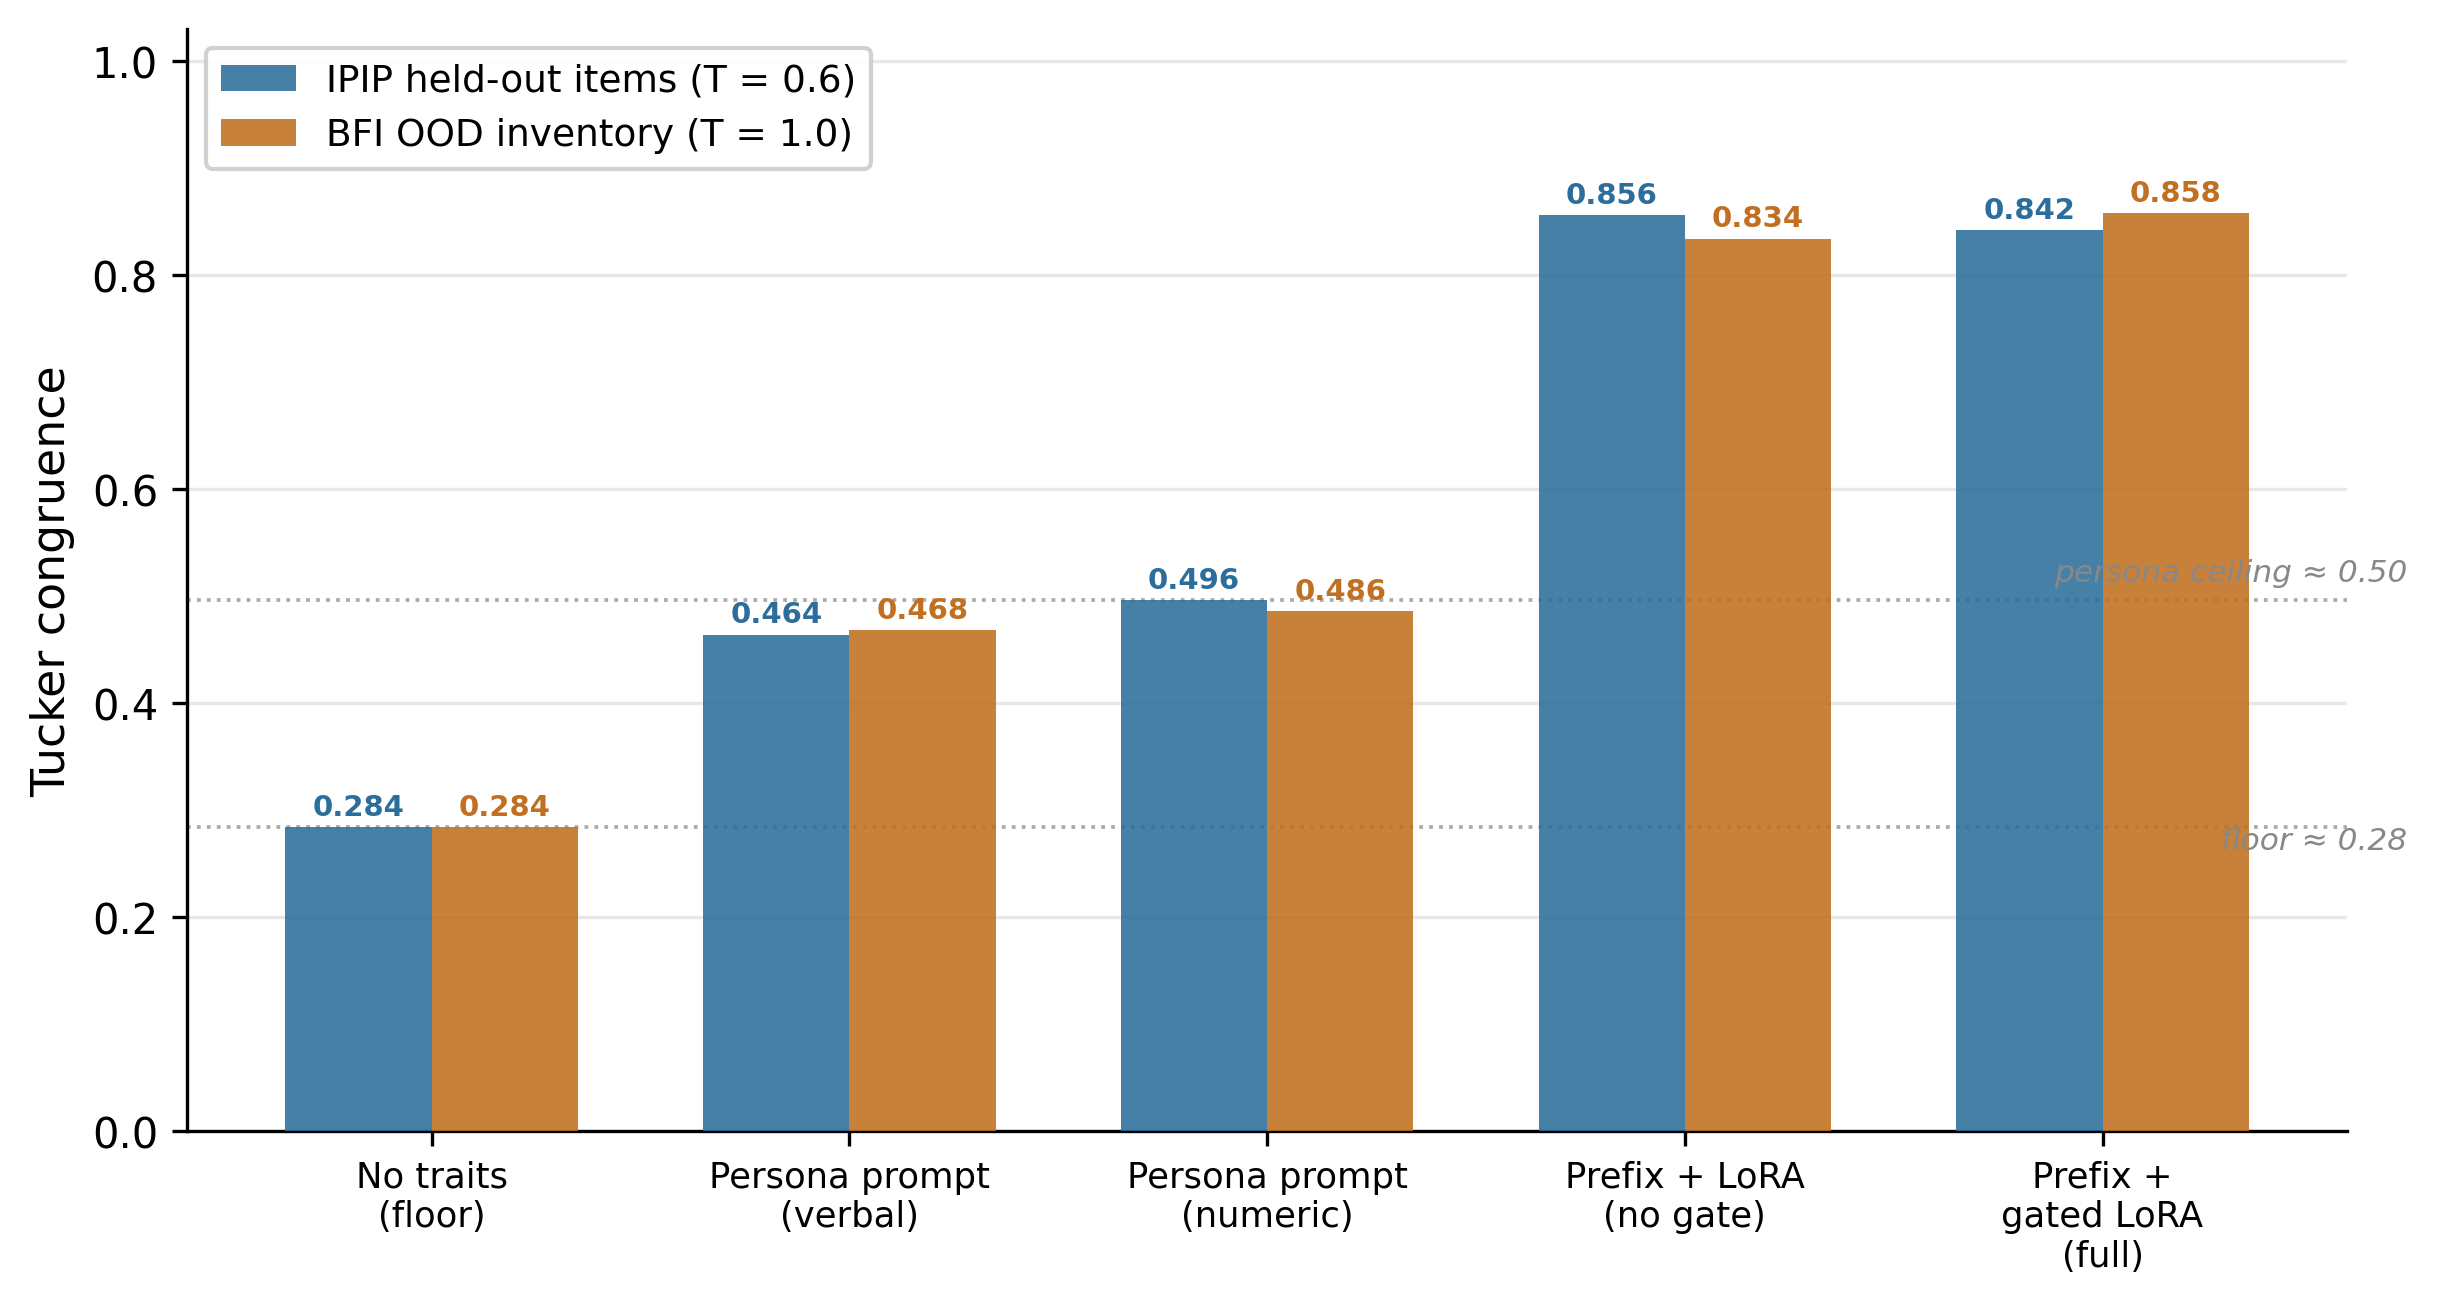
\includegraphics[width=\linewidth]{figures/fig2_ablation_bars.png}
\caption{Ablation ladder: Tucker factor congruence for each conditioning mode evaluated on IPIP
held-out items (blue) and BFI out-of-distribution inventory (orange). Dotted
reference lines mark the no-trait floor ($\approx$0.28) and the persona-prompt ceiling ($\approx$0.50).
Trained latent conditioning (rightmost two groups) nearly doubles persona-prompting; the latent gate
adds negligible benefit. All values from matched 3-epoch runs.}
\label{fig:ablation}
\end{figure}

From table 3 we can see that Baseline\_c and the full model are basically equivalent, we therefore do not claim latent gating as a contribution; the contributions are the prefix+LoRA continuous-latent conditioning, the sampling-based silicon-sample construction, and the validity evidence. We ship \texttt{full} as an operational choice (slightly better, more balanced OOD); baseline\_c is a near-equivalent simpler fallback.

\subsection{Criterion and nomological validity}

The structural analyses above show that silicon respondents reproduce human factor structure on held-out items. A complementary question is whether the population also recovers the relationships between personality and non-personality outcomes — what psychometric standards call criterion or nomological network validity. This matters particularly because the training setup carries a residual circularity: the conditioning latents are CFA factor scores from the IPIP data, and the inter-factor covariance $\Sigma_{\text{human}}$ is injected directly. Evidence that the model reproduces trait correlates that are absent from $\Sigma_{\text{human}}$ and from the training items would indicate genuine construct-to-response learning rather than injected covariance replay.

To test this we administered four instruments from outside the personality domain whose Big Five correlates are established in the meta-analytic literature: the Grit-S scale (8 items; dominant trait +C, \citep{duckworth2009}), the Rosenberg Self-Esteem Scale (10 items; dominant trait $-$N, \citep{robins2001}), a public-domain leadership emergence measure (10 items; dominant trait +E, \citep{judge2002}), and a procrastination scale (8 items; dominant trait $-$C, \citep{steel2007}). Twenty held-out IPIP Big Five marker items were also included to produce an observed trait score for each synthetic respondent alongside the injected latent z. The battery was administered to n = 1000 synthetic respondents drawn from $\mathcal{N}(\boldsymbol{\mu}_{\text{human}}, \Sigma_{\text{human}})$ (Equation~\ref{eq:latents}) at T = 1.0; domain scores were correlated against the observed Big Five scale scores. The domain–trait relationships tested here are nowhere in $\Sigma_{\text{human}}$: the training procedure injects only the Big Five inter-factor structure, not any link between personality and grit, self-esteem, leadership, or procrastination.

Table 4 reports the silicon zero-order correlations alongside the meta-analytic targets. All four domains recover the correct sign on their theoretically dominant trait, with bootstrap 95\% CIs excluding zero on the dominant-trait correlation in every case. Profile correlations with the literature vectors range from 0.73 (procrastination) to 0.95 (self-esteem), with a mean of 0.87 (Qwen, n = 1000); Llama reaches similar result we chose to not report the result for brevity. The floor condition (baseline\_a, no traits) yields mean profile correlations near zero, confirming that the signal is produced by trait conditioning rather than by item content or the sampling procedure.

\begin{table}[ht!]
\centering
\caption{Silicon zero-order Pearson correlations between each domain score and observed Big Five scale scores (Qwen, n = 1000, T = 1.0), alongside the meta-analytic literature target vector used for validation (sources: \citep{duckworth2009,robins2001,judge2002,steel2007}). Profile r: Pearson correlation between the five-element silicon r-vector and the literature target vector. The theoretically dominant trait is in the expected direction for all four domains; bootstrap 95\% CIs on the dominant-trait correlation exclude zero in every case. The floor (baseline\_a, no traits) gives mean profile r $\approx$ 0.}
\resizebox{\textwidth}{!}{%
\begin{tabular}{lccccccc}
\toprule
Domain & Literature target (O / C / E / A / N) & Silicon $r_O$ & Silicon $r_C$ & Silicon $r_E$ & Silicon $r_A$ & Silicon $r_N$ & Profile r \\
\midrule
Grit (+C) & .06 / .77 / .20 / .24 / $-$.40 & +.39 & +.54 & +.21 & +.38 & $-$.36 & .88 \\
Self-esteem ($-$N) & .17 / .24 / .38 / .13 / $-$.50 & +.48 & +.52 & +.44 & +.47 & $-$.50 & .95 \\
Leadership (+E) & .24 / .28 / .31 / .08 / $-$.24 & +.49 & +.38 & +.65 & +.46 & $-$.07 & .91 \\
Procrastination ($-$C) & .03 / $-$.62 / $-$.12 / $-$.12 / .24 & $-$.38 & $-$.52 & $-$.36 & $-$.38 & +.56 & .73 \\
\bottomrule
\end{tabular}
}
\end{table}

A serious concern with the zero-order profile is that an evaluative halo — a shared positive loading on socially desirable traits and a negative one on Neuroticism — could inflate every correlation and manufacture apparent criterion validity without any genuine construct learning. Because the meta-analytic target vectors are themselves close to this halo shape, the profile-correlation metric has limited power to separate the two. We make this explicit with two reference baselines computed against the identical literature targets (Table~\ref{tab:criterion-baselines}). A \emph{pure halo} vector — $(+,+,+,+,-)$ on O/C/E/A/N, oriented a priori by domain valence and carrying no model information — attains a mean profile r of 0.82 versus the model's 0.87, and in fact matches or exceeds the model on Self-esteem and Leadership; it also reproduces the correct dominant-trait sign in all four domains by construction, so the ``correct sign in 36/36 cells'' headline carries little discriminating value. The model exceeds the halo only on Grit and Procrastination — the two domains whose literature profile is least halo-shaped (a single strong Conscientiousness loading). A second, \emph{semantic} baseline predicts each domain's trait profile from item text alone — embedding every battery item with the frozen backbone and taking the cosine between sign-keyed domain and trait directions — and reaches a mean profile r of only 0.35, well below both the model and the halo; item wording therefore does not by itself reproduce the profiles. Taken together, the zero-order profile correlation and the sign test are necessary but not sufficient. We therefore rest the nomological claim on the discriminant $\beta$ analysis below, which a halo cannot satisfy: we regress each domain score on all five Big Five predictors simultaneously (z-scored inputs and outcomes), yielding standardized $\beta$ coefficients that partial out the shared evaluative variance and isolate each factor's unique contribution.

\begin{table}[ht!]
\centering
\caption{Profile-correlation baselines for the criterion metric, against the identical meta-analytic literature targets. \textbf{Model}: silicon zero-order profile r (Qwen seed 0, n = 1000). \textbf{Halo}: a pure evaluative-halo vector $(+,+,+,+,-)$ oriented by domain valence, carrying no model information. \textbf{Semantic}: profile predicted from item text alone (frozen-backbone embeddings, sign-keyed domain-vs-trait cosine). \textbf{Floor}: no-trait baseline\_a. A pure halo nearly matches the model, exposing the metric's limited discriminating power; item semantics alone do not.}
\label{tab:criterion-baselines}
\begin{tabular}{lcccc}
\toprule
Domain & Model & Halo & Semantic & Floor \\
\midrule
Grit & 0.88 & 0.77 & 0.14 & $-$0.12 \\
Self-esteem & 0.95 & 0.96 & 0.57 & 0.11 \\
Leadership & 0.91 & 0.92 & 0.25 & $-$0.22 \\
Procrastination & 0.73 & 0.63 & 0.44 & 0.24 \\
\midrule
Mean & 0.87 & 0.82 & 0.35 & 0.01 \\
\bottomrule
\end{tabular}
\end{table}

Table 5 reports the standardized $\beta$ coefficients across all trained models (five Qwen seeds, four Llama seeds; n = 9; Figure~\ref{fig:criterion-betas}). The discriminant evidence is strongest here, because -- unlike the zero-order profile, which a pure evaluative halo can already reproduce (Table~\ref{tab:criterion-baselines}) -- a halo cannot produce single-trait $\beta$ dominance. Across all 36 model $\times$ domain cells the dominant-trait $\beta$ carries the correct sign in every case, and it is the largest-magnitude $\beta$ (argmax) in 27 (75\%); but this figure splits cleanly by domain into two strong single-trait cases and two weaker multi-trait cases, as the three patterns below make explicit.

For Grit and Leadership the $\beta$ picture is unambiguous: the dominant trait is the $\beta$-argmax in all nine checkpoints (9/9 each; C for Grit, E for Leadership), with the target coefficient at least 0.10 larger in magnitude than the next-largest. These are single-trait dominance patterns that a generic halo cannot generate, and they match the respective meta-analytic findings; it is these two domains that carry the discriminant-validity claim.

For Procrastination the evidence is weaker: $\beta_C$ dominates $\beta_N$ in the mean ($-$0.37 vs +0.35), matching \citet{steel2007}'s finding that Conscientiousness is the strongest predictor and Neuroticism secondary, but Conscientiousness is the per-checkpoint $\beta$-argmax in only 5 of 9 checkpoints, so we do not claim clean single-trait dominance here.

For Self-esteem the evidence is likewise weaker but interpretable: the $\beta$ pattern reproduces the three-trait loading reported by \citet{robins2001}, with N most negative alongside substantial and comparable E and C contributions. $\beta_N$ CIs exclude zero on every checkpoint (mean $\beta_N$ = $-$0.29 $\pm$ 0.08), so Neuroticism's unique contribution is statistically isolated throughout; but N is the $\beta$-argmax in only 4 of 9 checkpoints, reflecting the near-equality of |$\beta_N$|, |$\beta_E$|, and |$\beta_C$|. We read this as the published multi-trait structure for self-esteem rather than clean discriminant dominance — consistent with the construct, but not, on its own, decisive against a halo account.

\begin{table}[ht!]
\centering
\caption{Standardized $\beta$ coefficients from multiple regression of each domain score on all five Big Five predictors simultaneously (z-scored inputs and outcomes). Values are mean $\pm$ SD across all trained checkpoints (five Qwen seeds, four Llama-3-8B-4bit seeds; n = 9). Target: the theoretically dominant trait and direction per meta-analytic literature. Argmax match: fraction of checkpoints where the largest-magnitude $\beta$ corresponds to the target trait. R$^2$: mean variance explained. The target-trait $\beta$ CI excludes zero in every domain.}
\resizebox{\textwidth}{!}{%
\begin{tabular}{lcccccccc}
\toprule
Domain & Target & $\beta_O$ & $\beta_C$ & $\beta_E$ & $\beta_A$ & $\beta_N$ & Argmax match & R$^2$ \\
\midrule
Grit & +C & +0.16 $\pm$ 0.03 & +0.36 $\pm$ 0.06 & +0.14 $\pm$ 0.04 & +0.14 $\pm$ 0.03 & $-$0.18 $\pm$ 0.05 & 9/9 & 0.43 \\
Self-esteem & $-$N & +0.17 $\pm$ 0.04 & +0.27 $\pm$ 0.05 & +0.29 $\pm$ 0.02 & +0.16 $\pm$ 0.04 & $-$0.29 $\pm$ 0.08 & 4/9 & 0.57 \\
Leadership & +E & +0.25 $\pm$ 0.02 & +0.26 $\pm$ 0.05 & +0.44 $\pm$ 0.06 & +0.16 $\pm$ 0.04 & +0.08 $\pm$ 0.05 & 9/9 & 0.57 \\
Procrastination & $-$C & $-$0.06 $\pm$ 0.04 & $-$0.37 $\pm$ 0.06 & $-$0.22 $\pm$ 0.05 & $-$0.07 $\pm$ 0.02 & +0.35 $\pm$ 0.06 & 5/9 & 0.53 \\
\bottomrule
\end{tabular}
}
\end{table}

\begin{figure}[ht!]
\centering
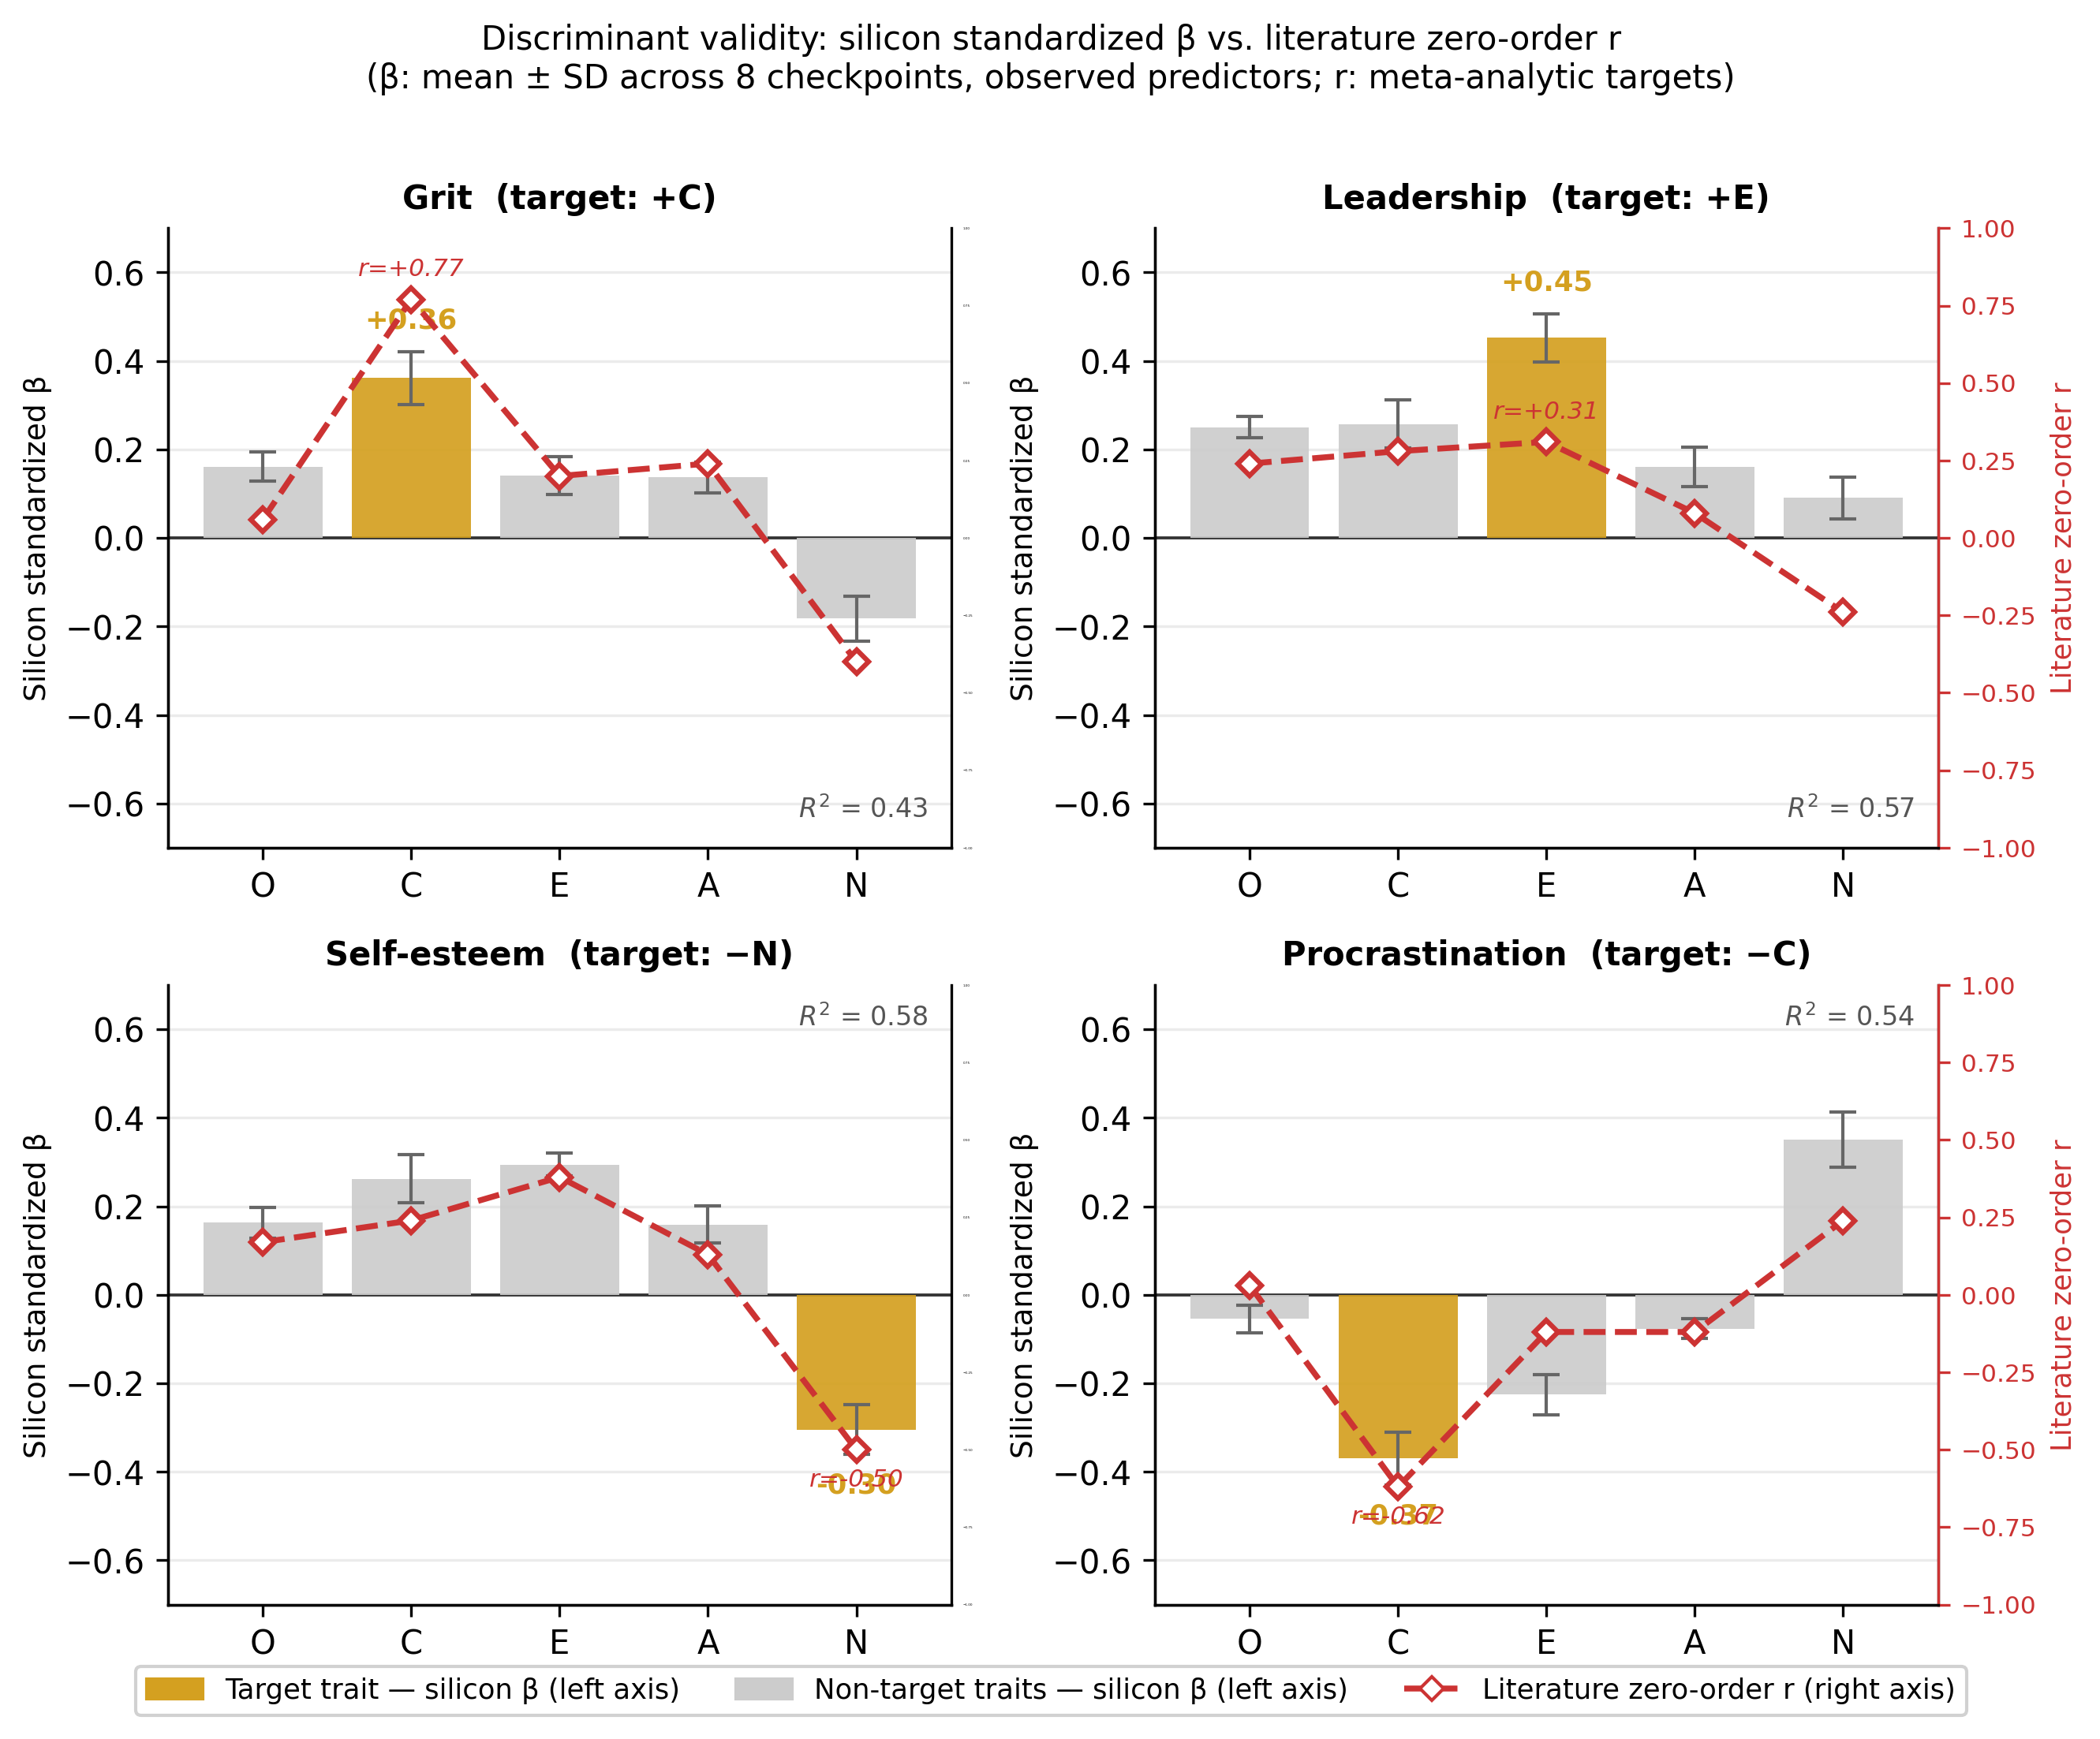
\includegraphics[width=\linewidth]{figures/fig4_criterion_betas.png}
\caption{Discriminant validity: silicon standardized $\beta$ profiles (bars) vs.\ meta-analytic
literature zero-order $r$ values (dashed line) for each criterion domain. Amplitude difference
between bars and line reflects variance partialling (betas control for inter-trait correlations;
zero-order $r$ does not). Profile shapes match in every domain: $C$ dominant for Grit, $E$
dominant for Leadership, $N$ most negative for Self-esteem alongside substantial $E$ and $C$
contributions matching the three-trait pattern in \citealt{robins2001}, and $C$-dominant with
secondary $N$ for Procrastination \citep{steel2007}. Values are means across nine checkpoints;
error bars show cross-checkpoint SD.}
\label{fig:criterion-betas}
\end{figure}


\subsection{Effects of Temperature on the Silicon Samples}

Here we analyze how the temperature, the fundamental parameter to control the level of stochasticity of the LLMs, influence the sampling generations.

For each of nine trained models $\times$ two inventories (IPIP, BFI), the human respondent pool is split 50/50 by deterministic permutation into a calibration half and a reporting half. Silicon responses are generated from scratch at nine temperatures (T $\in$ {0.4, 0.5, \ldots{}, 1.2}) against the full silicon population (n = 1000). The calibration half selects $T^*$ by minimising a moment-match objective: the per-item root mean squared difference between the human and silicon response distributions in their mean and standard deviation (BFI rescaled to 1–5 for comparability). The reporting half is used for all the metrics and never informs T selection.

Table 6 shows the calibration-optimal $T^*$ and the calibration objective value at $T^*$, aggregated (mean $\pm$ SD) across seeds. In all four backbone $\times$ inventory configurations, mean $T^*$ falls at 1.12–1.20  with SD $\leq$ 0.05, i.e. essentially every individual seed selects the same calibration-optimal temperature. The calibration objective decreases monotonically across the grid: at low temperatures silicon per-item response distributions are over-peaked relative to humans (the model concentrates probability more sharply on a few Likert options than humans do), and raising T broadens the marginal until the silicon spread matches human spread.

\begin{table}[ht!]
\centering
\caption{Calibration-optimal temperature $T^*$ selected by moment-match on the calibration half of human respondents, aggregated across seeds (mean $\pm$ SD). The calibration objective is per-item mean+std RMSE between human and silicon response distributions (lower is better).}
\resizebox{\textwidth}{!}{%
\begin{tabular}{lccccc}
\toprule
Backbone (n) & Inventory  & Mean $T^*$ & SD $T^*$ & Mean calib. obj at $T^*$ & SD calib. obj \\
\midrule
Qwen & IPIP & 1.20 & 0.00 & 0.537 & 0.034 \\
Qwen & BFI  & 1.12 & 0.05 & 0.394 & 0.022 \\
Llama & IPIP & 1.20 & 0.00 & 0.518 & 0.054 \\
Llama & BFI & 1.20 & 0.00 & 0.421 & 0.043 \\
\bottomrule
\end{tabular}
}
\end{table}

Table 7 shows Tucker congruence on the reporting half across the full temperature grid, aggregated across seeds. The key observation is that Tucker varies little with T: the aggregate mean spread across T $\in$ [0.4, 1.2] ranges from 0.015 $\pm$ 0.007 (Qwen IPIP) to 0.046 $\pm$ 0.008 (Llama IPIP). Factor structure is essentially T-invariant over this range. Intuitively, Tucker congruence depends on item-item correlations, a correlation is unchanged by an affine rescaling of either variable, and within this range T acts approximately as such a rescaling of each item's marginal spread, leaving the across-respondent co-variation that the structure depends on largely intact. The near-invariance is empirical and local to this range rather than exact.

\begin{table}[ht!]
\centering
\caption{Tucker congruence on the reporting half of human respondents across five representative temperatures, mean $\pm$ SD across seeds. Mean spread = mean across seeds of (max $-$ min) across the full grid T $\in$ [0.4, 1.2]. All mean spreads are within or close to the cross-seed SD in \S{}5.5.}
\resizebox{\textwidth}{!}{%
\begin{tabular}{lcccccc}
\toprule
Backbone $\times$ inventory (n) & T=0.4 & T=0.6 & T=0.8 & T=1.0 & T=1.2 & Mean spread \\
\midrule
Qwen $\times$ IPIP & 0.861 $\pm$ 0.010 & 0.867 $\pm$ 0.006 & 0.870 $\pm$ 0.009 & 0.872 $\pm$ 0.003 & 0.868 $\pm$ 0.010 & 0.015 $\pm$ 0.007 \\
Qwen $\times$ BFI & 0.869 $\pm$ 0.010 & 0.865 $\pm$ 0.009 & 0.862 $\pm$ 0.013 & 0.858 $\pm$ 0.017 & 0.849 $\pm$ 0.014 & 0.021 $\pm$ 0.007 \\
Llama $\times$ IPIP & 0.900 $\pm$ 0.035 & 0.898 $\pm$ 0.029 & 0.888 $\pm$ 0.029 & 0.877 $\pm$ 0.033 & 0.861 $\pm$ 0.035 & 0.046 $\pm$ 0.008 \\
Llama $\times$ BFI & 0.855 $\pm$ 0.043 & 0.847 $\pm$ 0.044 & 0.837 $\pm$ 0.052 & 0.831 $\pm$ 0.048 & 0.820 $\pm$ 0.056 & 0.035 $\pm$ 0.013 \\
\bottomrule
\end{tabular}
}
\end{table}

At the calibration-optimal $T^*$, the aggregate mean Tucker change relative to the prior eval-tuned T is small in every cell and not uniformly signed: Qwen IPIP $\Delta$ = +0.001 $\pm$ 0.005, Qwen BFI $\Delta$ = $-$0.004 $\pm$ 0.003, Llama IPIP $\Delta$ = $-$0.038 $\pm$ 0.006, Llama BFI $\Delta$ = $-$0.012 $\pm$ 0.007. The largest aggregate drop (Llama IPIP) matches the single largest per-seed drop seen in any individual checkpoint ($-$0.034 to $-$0.048), so the original two-checkpoint analysis was not an unrepresentative pick — the effect replicates at the same small magnitude across all four healthy Llama seeds. As an illustrative single-checkpoint check, the criterion mean profile correlation at the BFI-optimal $T^*$ = 1.10 (Qwen seed 0) is 0.866, identical to the \S{}5.4 value at the prior T = 1.0.

Temperature therefore plays two distinct roles that do not interact. It is a marginal-distribution calibration knob: changing T adjusts per-item response spread so that silicon distributions resemble human distributions, and the calibration objective selects the T that minimises this mismatch. Separately, it is not a factor-structure knob: the Tucker congruence and criterion validity that constitute the paper's headline claims are robust across the full temperature grid and do not depend on the specific T chosen during initial evaluation.

\subsection{Generative stability and internal consistency}

We report two complementary measures: generative (sampling) stability across repeated administrations and internal consistency (Cronbach $\alpha$) within a single administration. We deliberately avoid the term \emph{test-retest reliability} here: human test-retest additionally reflects occasion and trait/state variation over time, whereas our procedure fixes the latent and re-runs only the categorical draw, isolating generative noise alone (see below).

The respondent population is held fixed at n = 500 latents z drawn once and saved. Each instrument is administered twice under different response-sampling seeds, keeping z, items, and checkpoint identical. The two administrations therefore differ only in the categorical sampling noise applied to each item's digit distribution — the sole stochastic step in silicon\_sample. Correlating reverse-coded scale scores across the 500 respondents gives a per-factor Pearson r that measures generative stability: how reproducibly the same latent z maps to the same scale score when the sampling is rerun.

All trained models are evaluated (five Qwen seeds, five Llama seeds), each on IPIP  and BFI . Tables 8 and 9 report per-factor generative-stability r and Cronbach $\alpha$ respectively, aggregated as mean $\pm$ SD across seeds within each model. Administrations 1 and 2 produced near-identical $\alpha$ values in all cells (within 0.06), confirming internal consistency is stable across sampling noise.

\begin{table}[ht!]
\centering
\caption{Silicon generative (sampling) stability: mean $\pm$ SD across seeds of the Pearson r between reverse-coded scale scores from two independent administrations with the same 500 fixed latents z per configuration. Values reflect generative-stability reliability — variability from categorical sampling noise only. O = Openness, C = Conscientiousness, E = Extraversion, A = Agreeableness, N = Neuroticism. Mean = unweighted mean across the five factors.}
\resizebox{\textwidth}{!}{%
\begin{tabular}{lcccccc}
\toprule
Config & O & C & E & A & N & Mean \\
\midrule
Qwen $\times$ IPIP & 0.69 $\pm$ 0.04 & 0.77 $\pm$ 0.02 & 0.89 $\pm$ 0.02 & 0.74 $\pm$ 0.05 & 0.80 $\pm$ 0.04 & 0.78 \\
Qwen $\times$ BFI & 0.57 $\pm$ 0.07 & 0.59 $\pm$ 0.02 & 0.77 $\pm$ 0.01 & 0.71 $\pm$ 0.03 & 0.82 $\pm$ 0.00 & 0.69 \\
Llama $\times$ IPIP & 0.68 $\pm$ 0.03 & 0.71 $\pm$ 0.03 & 0.84 $\pm$ 0.03 & 0.83 $\pm$ 0.01 & 0.84 $\pm$ 0.02 & 0.78 \\
Llama $\times$ BFI & 0.61 $\pm$ 0.02 & 0.55 $\pm$ 0.04 & 0.70 $\pm$ 0.02 & 0.73 $\pm$ 0.04 & 0.85 $\pm$ 0.01 & 0.69 \\
\bottomrule
\end{tabular}
}
\end{table}

\begin{table}[ht!]
\centering
\caption{Cronbach $\alpha$: mean $\pm$ SD across seeds. Scale lengths: IPIP the 4 held-out items per factor, BFI 5 items per factor.}
\resizebox{\textwidth}{!}{%
\begin{tabular}{lcccccc}
\toprule
Config & O & C & E & A & N & Mean \\
\midrule
Qwen $\times$ IPIP & 0.48 $\pm$ 0.05 & 0.68 $\pm$ 0.02 & 0.84 $\pm$ 0.02 & 0.58 $\pm$ 0.06 & 0.71 $\pm$ 0.06 & 0.66 \\
Qwen $\times$ BFI & 0.46 $\pm$ 0.08 & 0.54 $\pm$ 0.02 & 0.72 $\pm$ 0.01 & 0.73 $\pm$ 0.03 & 0.82 $\pm$ 0.00 & 0.65 \\
Llama $\times$ IPIP & 0.55 $\pm$ 0.05 & 0.61 $\pm$ 0.07 & 0.74 $\pm$ 0.05 & 0.74 $\pm$ 0.01 & 0.78 $\pm$ 0.02 & 0.68 \\
Llama $\times$ BFI & 0.51 $\pm$ 0.04 & 0.51 $\pm$ 0.04 & 0.66 $\pm$ 0.03 & 0.73 $\pm$ 0.04 & 0.84 $\pm$ 0.01 & 0.65 \\
\bottomrule
\end{tabular}
}
\end{table}

Four findings emerge. First, silicon generative-stability r and Cronbach $\alpha$ are of broadly similar magnitude to values reported for published short-form Big Five inventories in human samples (test-retest r typically 0.65–0.85; $\alpha$ typically 0.50–0.85 for 4–5 item scales); the mean stability r across all four configurations ranges from 0.69 to 0.78. We stress that this is an orienting comparison, not a construct-equivalent one: human test-retest reliability additionally reflects occasion and trait/state variation across sessions, whereas our quantity fixes the latent and varies only the categorical sampling, so it isolates generative noise and is itself tunable via temperature (Finding 4; \S{}5.6). The similarity therefore indicates that the population is neither deterministic nor unstable — not that the simulator reproduces human test-retest reliability per se. Second, the cross-seed SDs are small for most factors, indicating that generative stability is a consistent property of the training process. The largest variance appears on Qwen BFI Openness (0.57 $\pm$ 0.07) and Qwen IPIP Agreeableness (0.74 $\pm$ 0.05), factors that also show wider structural variance in \S{}5.1–\S{}5.2. Third, the factor-level ordering is consistent across both backbones and both measures: Extraversion and Neuroticism are the most stable factors, Openness is the least stable on IPIP, and Conscientiousness joins Openness at the bottom on BFI. This mirrors the reliability ordering seen in human short-form inventories. Fourth, Qwen and Llama show nearly identical mean stability r (both 0.78 on IPIP, both 0.69 on BFI), indicating that generative stability is determined primarily by the instrument and temperature rather than by LLM architecture.


\section{Discussion}

The results described in section \S{}5 form a chain of evidence rather than a single number, and the chain is what the argument rests on. Taken individually, any one link could be explained away: a Tucker congruence of 0.85 on held-out items could reflect memorized item-response patterns rather than a learned construct; transfer to the BFI could reflect surface overlap between the two inventories' wording; the criterion correlations could reflect a generic evaluative halo; the multi-seed numbers could reflect a single lucky hyperparameter setting; the temperature used to generate every other table could itself be a tuned artifact. Taken together, the links close off these explanations one at a time. Cross-inventory transfer  rules out item memorization, since the BFI's 25 items share no text with the IPIP training items and use a different response scale (1–6 vs 1–5); a model that had merely memorized IPIP item-response statistics would have no mechanism for producing the right factor structure on wording it has never seen. The criterion battery rules out replay of the injected covariance $\Sigma_{\text{human}}$, since the domain–trait relationships tested there — grit with conscientiousness, self-esteem with neuroticism, leadership with extraversion, procrastination with conscientiousness — are absent from $\Sigma_{\text{human}}$ by construction; the training procedure injects only the Big Five inter-factor structure, never a personality–outcome link. A model that recovers those links could in principle be exploiting a generic evaluative halo rather than construct knowledge — and indeed a pure halo vector matches the zero-order profile correlations and the 36-of-36 sign pattern almost as well as the model does, so those two statistics are necessary but not sufficient. What a halo cannot produce is single-trait discriminant structure under simultaneous regression, and this is exactly what appears for grit (Conscientiousness the largest $\beta$ in 9 of 9 checkpoints) and leadership (Extraversion, 9 of 9); for self-esteem and procrastination the target trait's unique contribution is statistically isolated (its $\beta$ confidence interval excludes zero on every checkpoint) but not consistently dominant (argmax in 4 of 9 and 5 of 9), matching the multi-trait patterns those two constructs show in the literature. The claim beyond covariance replay therefore rests on the two single-trait domains, with the other two consistent-with-literature but weaker. The nine-checkpoint replication rules out single-run or single-backbone luck, since the headline numbers reproduce within a few hundredths of Tucker congruence across all Qwen seeds and Llama-3-8B seeds — a substantially larger model with a different tokenizer, architecture, and pretraining corpus. The held-out temperature calibration rules out the headline numbers being an artifact of hand-tuning T against the same data used to report Tucker congruence, since selecting T on a disjoint calibration half of the human sample and reporting on the other half changes Tucker congruence by at most a few hundredths in either direction, and the calibration-optimal temperature is consistently higher than the temperature originally chosen by inspection — meaning the original choice, if anything, understated rather than inflated the headline numbers. The reliability analysis addresses a different kind of concern: even a genuinely construct-valid synthetic population is not useful for downstream survey methodology if its measurement properties look nothing like a real instrument's. Silicon generative-stability correlations and Cronbach alphas are of broadly similar magnitude to those reported for published human short-form Big Five inventories (an orienting rather than construct-equivalent comparison, since our quantity isolates sampling noise and is temperature-tunable), and the factor-level ordering of stability — extraversion and neuroticism most stable, openness least — mirrors the ordering of reliability seen in human samples. A simulator that reproduced factor structure but had, say, near-perfect or near-zero generative stability would be a poor stand-in for a human population even if its Tucker congruence looked identical on paper; the fact that the noise properties also resemble a real instrument is part of the validity case, not a separate result.

It is worth to note that the gate ablation  shows that the latent gating mechanism we built into the architecture — a sigmoid gate over the LoRA bottleneck, modulated by the trait code — does not produce so much difference: gated and ungated variants differ by about 0.02 Tucker congruence in opposite directions on IPIP versus BFI. We report this transparently because it reallocates where we believe the paper's contribution actually lives: not in the gating mechanism, but in the combination of continuous soft-prefix and LoRA conditioning, the sampling-based (rather than argmax) construction of the silicon population, and the validity battery itself.

Positioned against the broader silicon-sampling literature, this work shares the goal of \citet{argyle2023}'s algorithmic-fidelity argument and the persona-prompting line of work \citep{serapiogarcia2023,jiang2023} — using language models to stand in for human respondents — but targets a different and, we think, more demanding bar: not whether prompted or conditioned trait scores correlate with intended traits, but whether a synthetic population built from such a model reproduces the factor structure, cross-instrument transfer, and nomological network that define a construct in the psychometric sense, and does so with the kind of statistical replication and robustness checks the methodology requires before the resulting synthetic data could be used for actual scale development or pilot testing. Relative to the persona-prompting baselines, trained latent conditioning nearly doubles factor congruence over the best zero-shot prompt format, which suggests that whatever silicon samples are capturing, it depends on more than the backbone's pre-existing capacity to role-play a description in context.


\section{Conclusion}

This paper describes and validates a method for building synthetic survey respondents that reproduce human Big Five psychometric structure: a frozen instruction language model conditioned on a continuous five-dimensional trait latent through a soft prefix and gated low-rank adapters, with each Likert response read directly from the model's own digit-token logits and sampled, rather than taken as an argmax, so that a synthetic population can be built whose item-level variability resembles a real respondent pool. Across nine trained checkpoints spanning two backbones (five Qwen and four Llama seeds), the resulting silicon populations attain fair factor congruence with the human five-factor structure on items withheld from training (mean Tucker $\approx$ 0.85, weakest on Neuroticism), transfer that structure to a different inventory with different item wording and a different response scale, partially recover the inter-factor correlation matrix (correct sign pattern, with a magnitude error that stays above the human split-half ceiling), and — most importantly for the validity argument — recover documented relationships between personality and four non-personality constructs that were never injected into the training procedure, with the correct correlation sign in every one of 36 checkpoint–domain cells and — the more demanding test, since a generic evaluative halo already reproduces that sign pattern — single-trait discriminant-regression structure for grit and leadership. These properties are robust to a held-out recalibration of the sampling temperature and are accompanied by generative-stability and internal-consistency statistics that are broadly comparable in magnitude to those reported for human short-form Big Five inventories, rather than being either implausibly perfect or unstable. An ablation shows that a gating mechanism added to the adapter architecture does not contribute measurably once training converges, so we attribute the method's contribution to the combination of continuous latent conditioning and sampling-based population construction rather than to any single architectural component.

These results make a reasonably strong case that the simulator is doing more than memorizing item statistics or replaying an injected correlation matrix, but several limitations bound how far that case extends. The conditioning latents used throughout are CFA factor scores derived from the same IPIP sample the model is trained on, and the inter-factor covariance $\Sigma_{\text{human}}$ used to draw the synthetic population is injected directly, so a degree of circularity is built into the setup by design; the emergent criterion validity in \S{}5.4 addresses this only partly, since it shows the recovered domain–trait links are not themselves injected, while the trait space they are expressed in still originates from the training inventory. Relatedly, criterion validity throughout this paper is benchmarked against meta-analytic literature targets rather than against a human sample in which the Big Five and the criterion instruments were measured together; a direct human-versus-silicon comparison on co-administered instruments would be a stronger test than comparison against a published correlation, and is the most valuable single follow-up this work points toward. Two factors are handled less well than the others, and for different reasons. Neuroticism has the lowest structural congruence on held-out items (0.74--0.76, below the ``fair'' threshold), and this is a genuine shortfall of the simulator rather than a limit of the construct or the analysis: on the identical items, two human subsamples recover Neuroticism at 0.98 (\S{}5.1), so the model is failing to reproduce structure that is clearly recoverable in humans. Openness, by contrast, is weakest not on congruence --- where it is in fact among the stronger factors (0.89--0.93) --- but on internal consistency and generative stability (lowest Cronbach $\alpha$ and lowest retest $r$ of the five factors); because that weakness mirrors Openness's comparatively low internal consistency in human normative data, we read it as a property of the construct the method is faithfully tracking rather than a defect of the architecture. We have not ruled out that targeted item augmentation could narrow either gap, and the Neuroticism gap in particular warrants it. Text-conditioned free generation is reliable on only one of the two backbones tested and was never directly supervised, so any production use of trait-conditioned text would need explicit text-level training rather than relying on this emergent transfer. Finally, the evidence base covers two inventories (IPIP and BFI) and a single construct family (the Big Five); whether the same conditioning approach and validity pattern would hold for other personality models, other psychological constructs, or instruments with substantially different item formats remains untested, and is the natural next axis along which to extend this work.


\section{Reproducibility}

All code, data splits, checkpoints, and per-checkpoint result tables are released. Key scripts: \texttt{train\_simulator.py}, \texttt{silicon\_sample.py}, \texttt{05\_simulator\_psychometrics.\{py,R\}}, \texttt{06\_criterion\_validity.py}, \texttt{07\_partial\_betas.py}, \texttt{08\_temp\_calibration.py}, \texttt{09\_text\_scoring.py}, \texttt{10\_reliability.py}, \texttt{train\_campaign.sh}, \texttt{eval\_campaign.py}. See \texttt{WALKTHROUGH.md} for the full result tables (\S{}7).
\bibliography{references}

\end{document}
